%\addcontentsline{toc}{chapter}{APPENDICES}             %toc entry  or:
%\addtocontents{toc}{\parindent0pt\vskip12pt APPENDICES} %toc entry, no page #

\section{Mesh Visualization}
\label{ch:app-paraview}

Paraview is program created by Kitware, Inc. which can visualize meshes
and fields on meshes.
It is the program of choice for viewing meshes created by the PUMI libraries.
The API \emph{m3dc1$\_$mesh$\_$write} writes a mesh either in ``smb" or ``vtk".

\begin{verbatim}
  // filename: output file name
  // option: 0 vtk file with field; 1 smb file
  m3dc1_mesh_write(char* filename, int *option)
\end{verbatim}\vspace{-.5cm}\hspace{1cm}

\begin{figure}
\centering
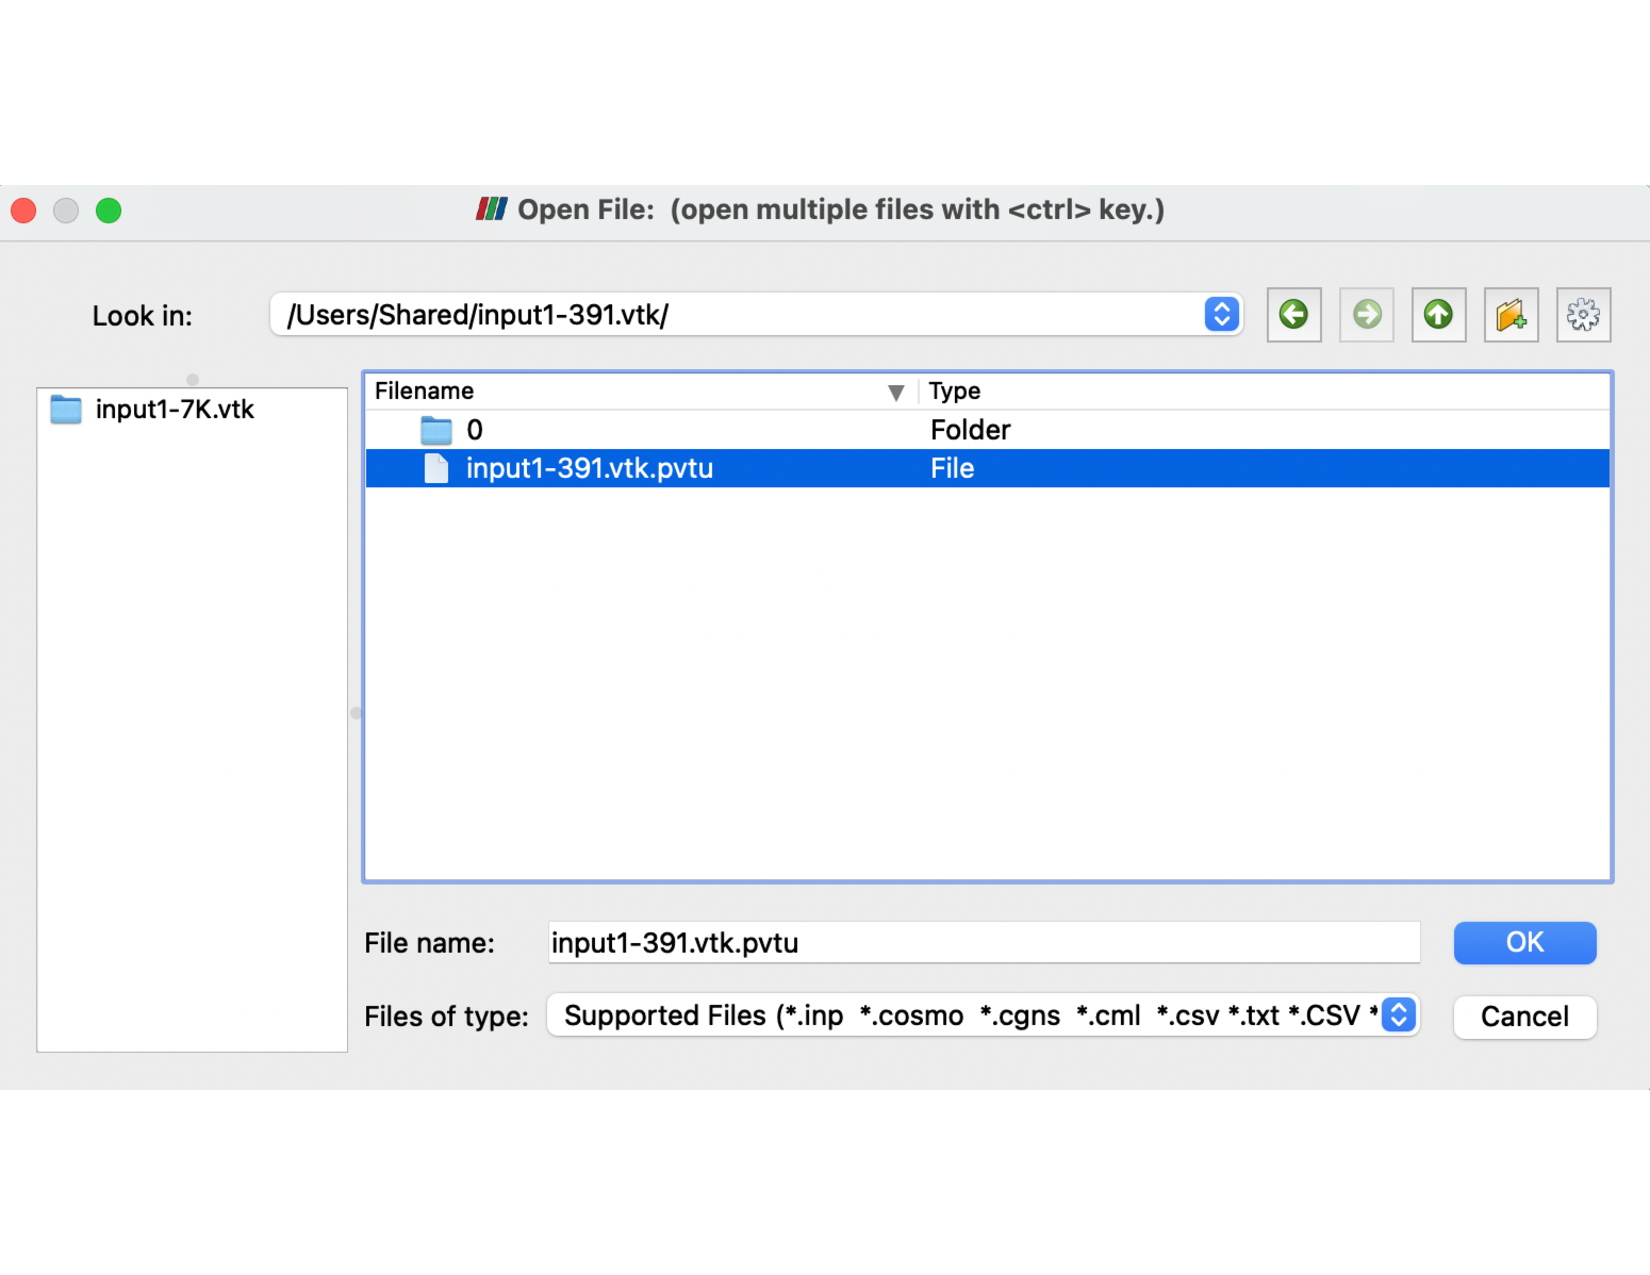
\includegraphics[width=3in]{./figures/paraview-fig1.pdf}
\caption{To visualize a mesh, select .pvtu file from Open File menu}
\label{fig:paraview-1}
\end{figure}

\begin{figure}
\centering
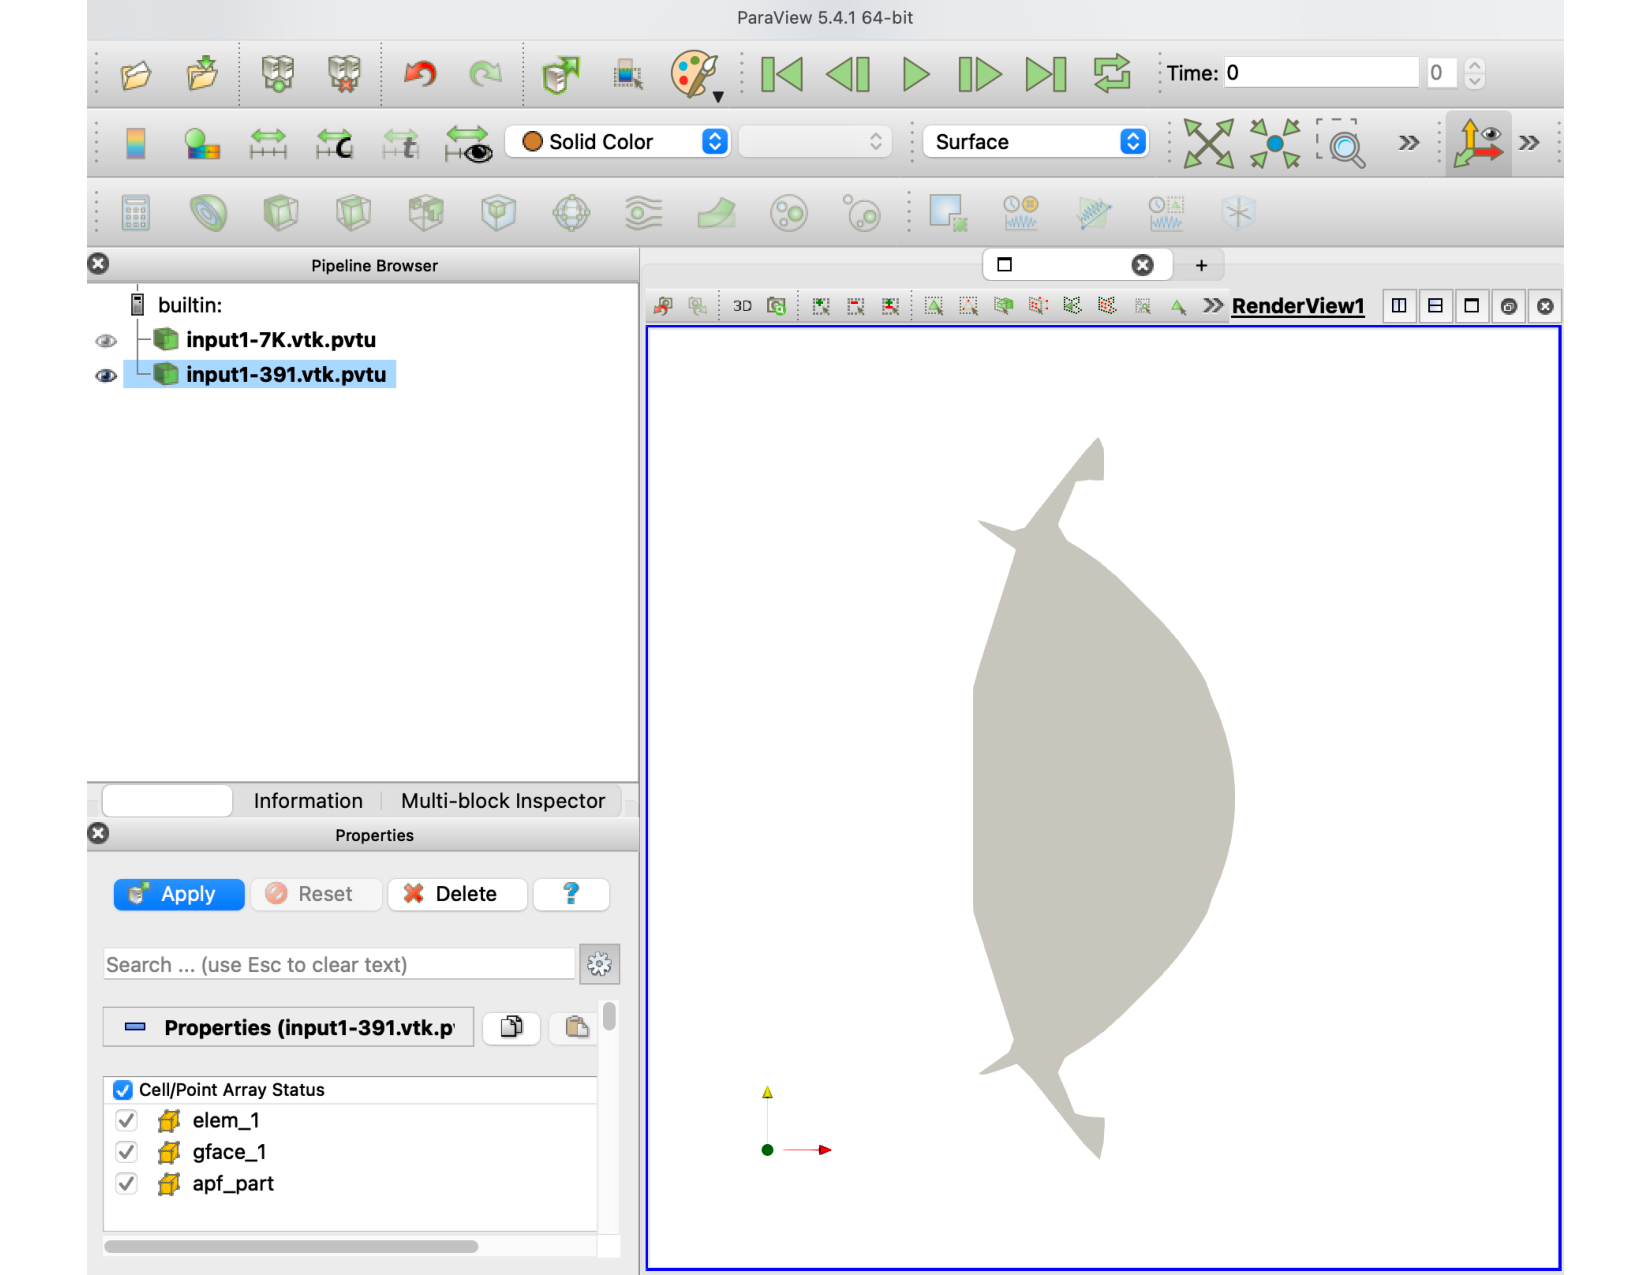
\includegraphics[width=4in]{./figures/paraview-fig2.pdf}
\caption{Initial Paraview window with a mesh}
\label{fig:paraview-2}
\end{figure}

\begin{figure}
\centering
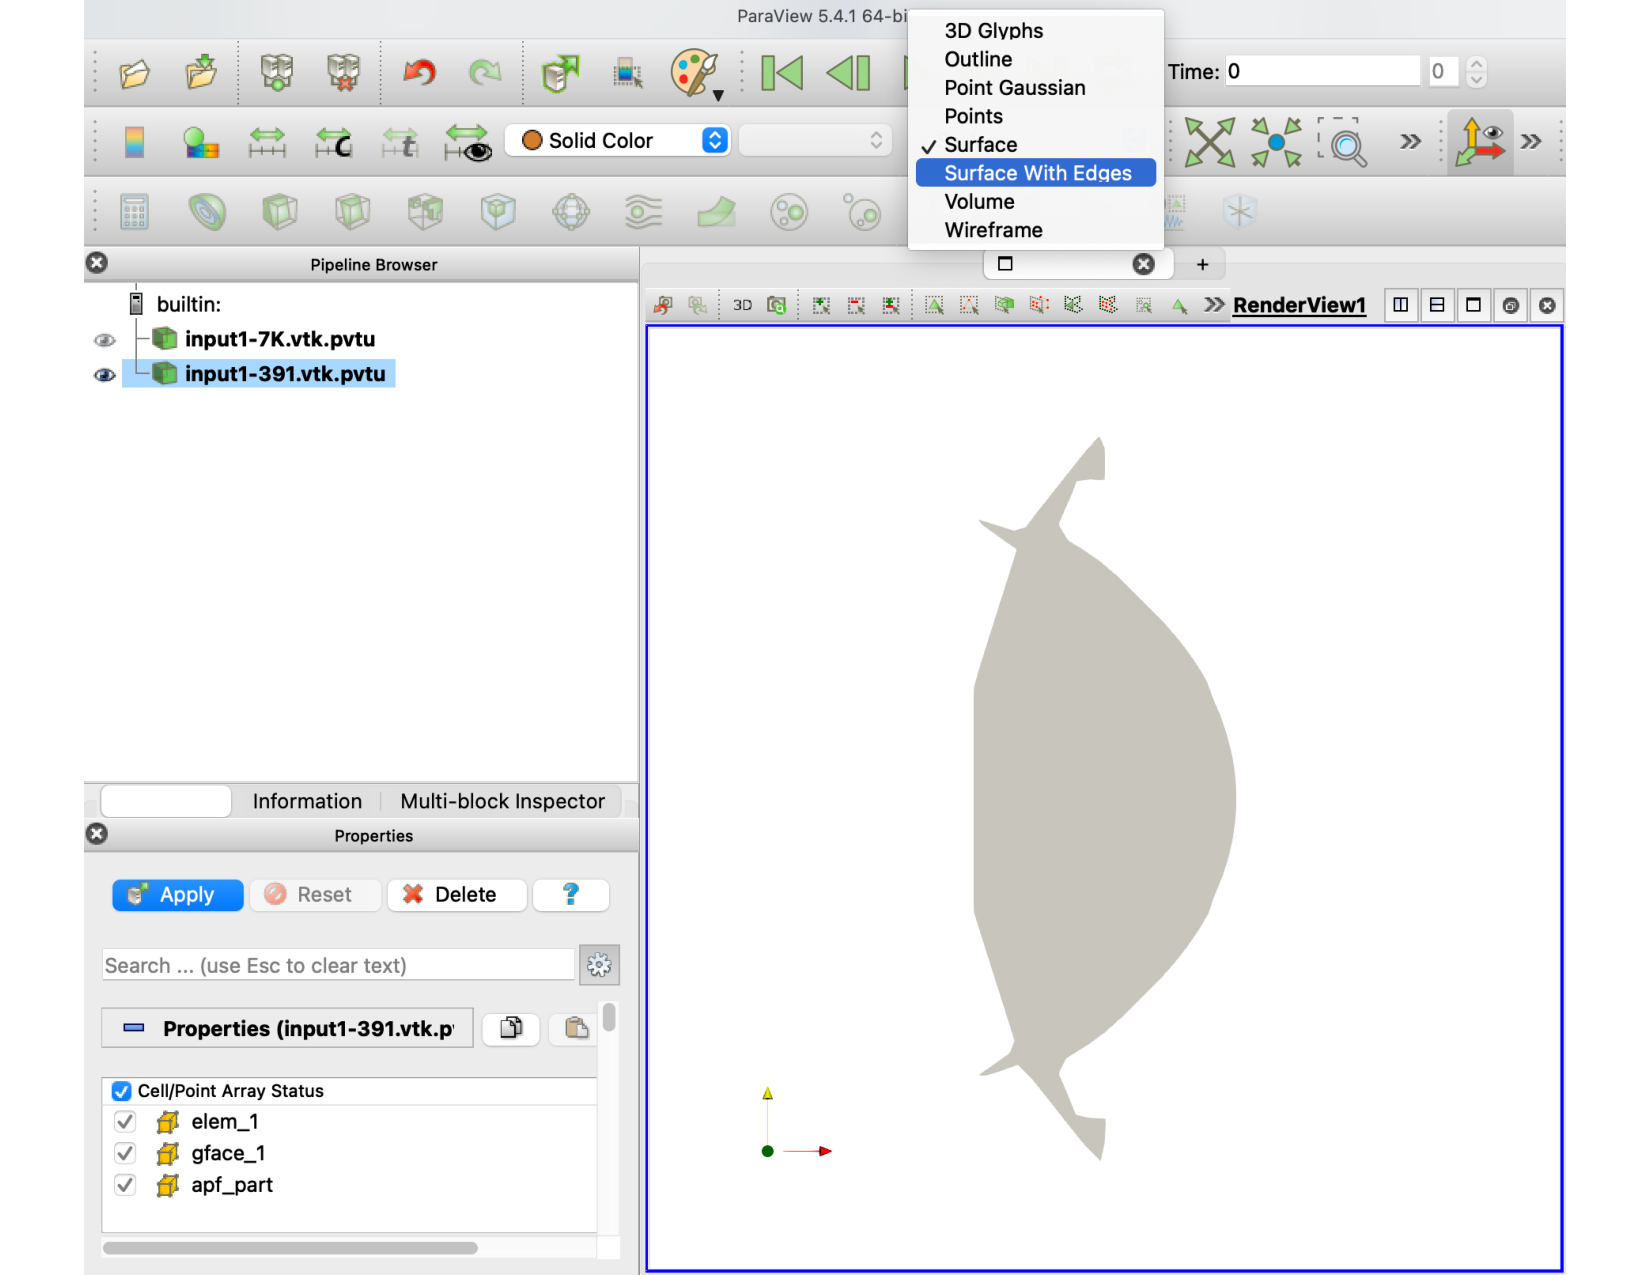
\includegraphics[width=4in]{./figures/paraview-fig3.pdf}
\caption{To render mesh decomposition, choose ``Surface With Edge"}
\label{fig:paraview-3}
\end{figure}


\begin{figure}
\centering
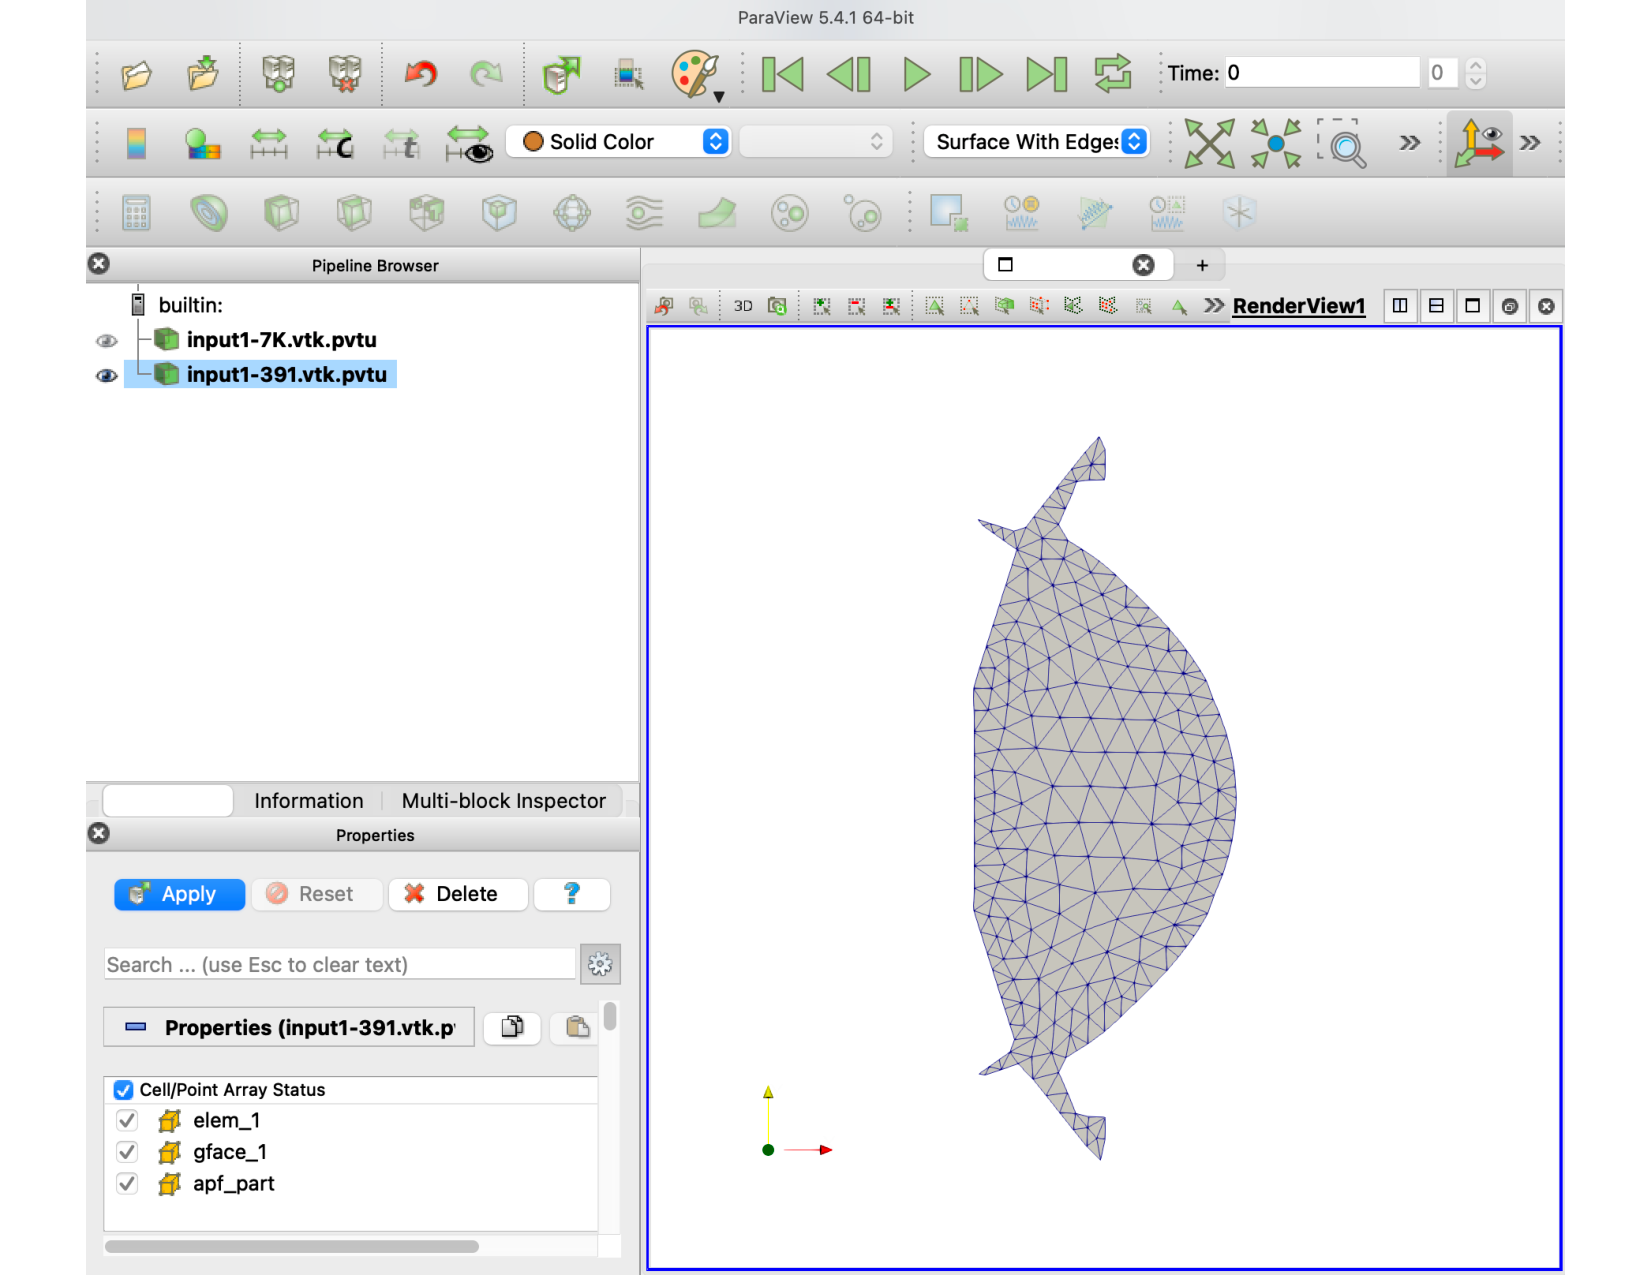
\includegraphics[width=4in]{./figures/paraview-fig4.pdf}
\caption{A mesh with ``Surface With Edge"}
\label{fig:paraview-4}
\end{figure}

If the first argument is ``output"" and the second argument is 0, filename is output, it creates the files \texttt{output.pvtu}. Opening the \texttt{output.pvtu} file in Paraview will show users the
mesh. Figures~\ref{fig:paraview-1} and ~\ref{fig:paraview-2} illustrate ``Open File" window and a mesh rendered in ``Surface" mode by default.


Changing ``Surface" to ``Surface with Edges" will outline each visible element.
Figures ~\ref{fig:paraview-3} and ~\ref{fig:paraview-4} illustrate how to make the decomposition visible.

Also, the mesh by default is rendered in one ``Solid Color".
There should be other options corresponding to the fields and numberings
that were on this mesh at the time of file writing.
There is an ``apf\_part" alternative for files written by APF, which
allows users to see the parallel partitioning of the mesh in color.

\begin{figure}
\centering
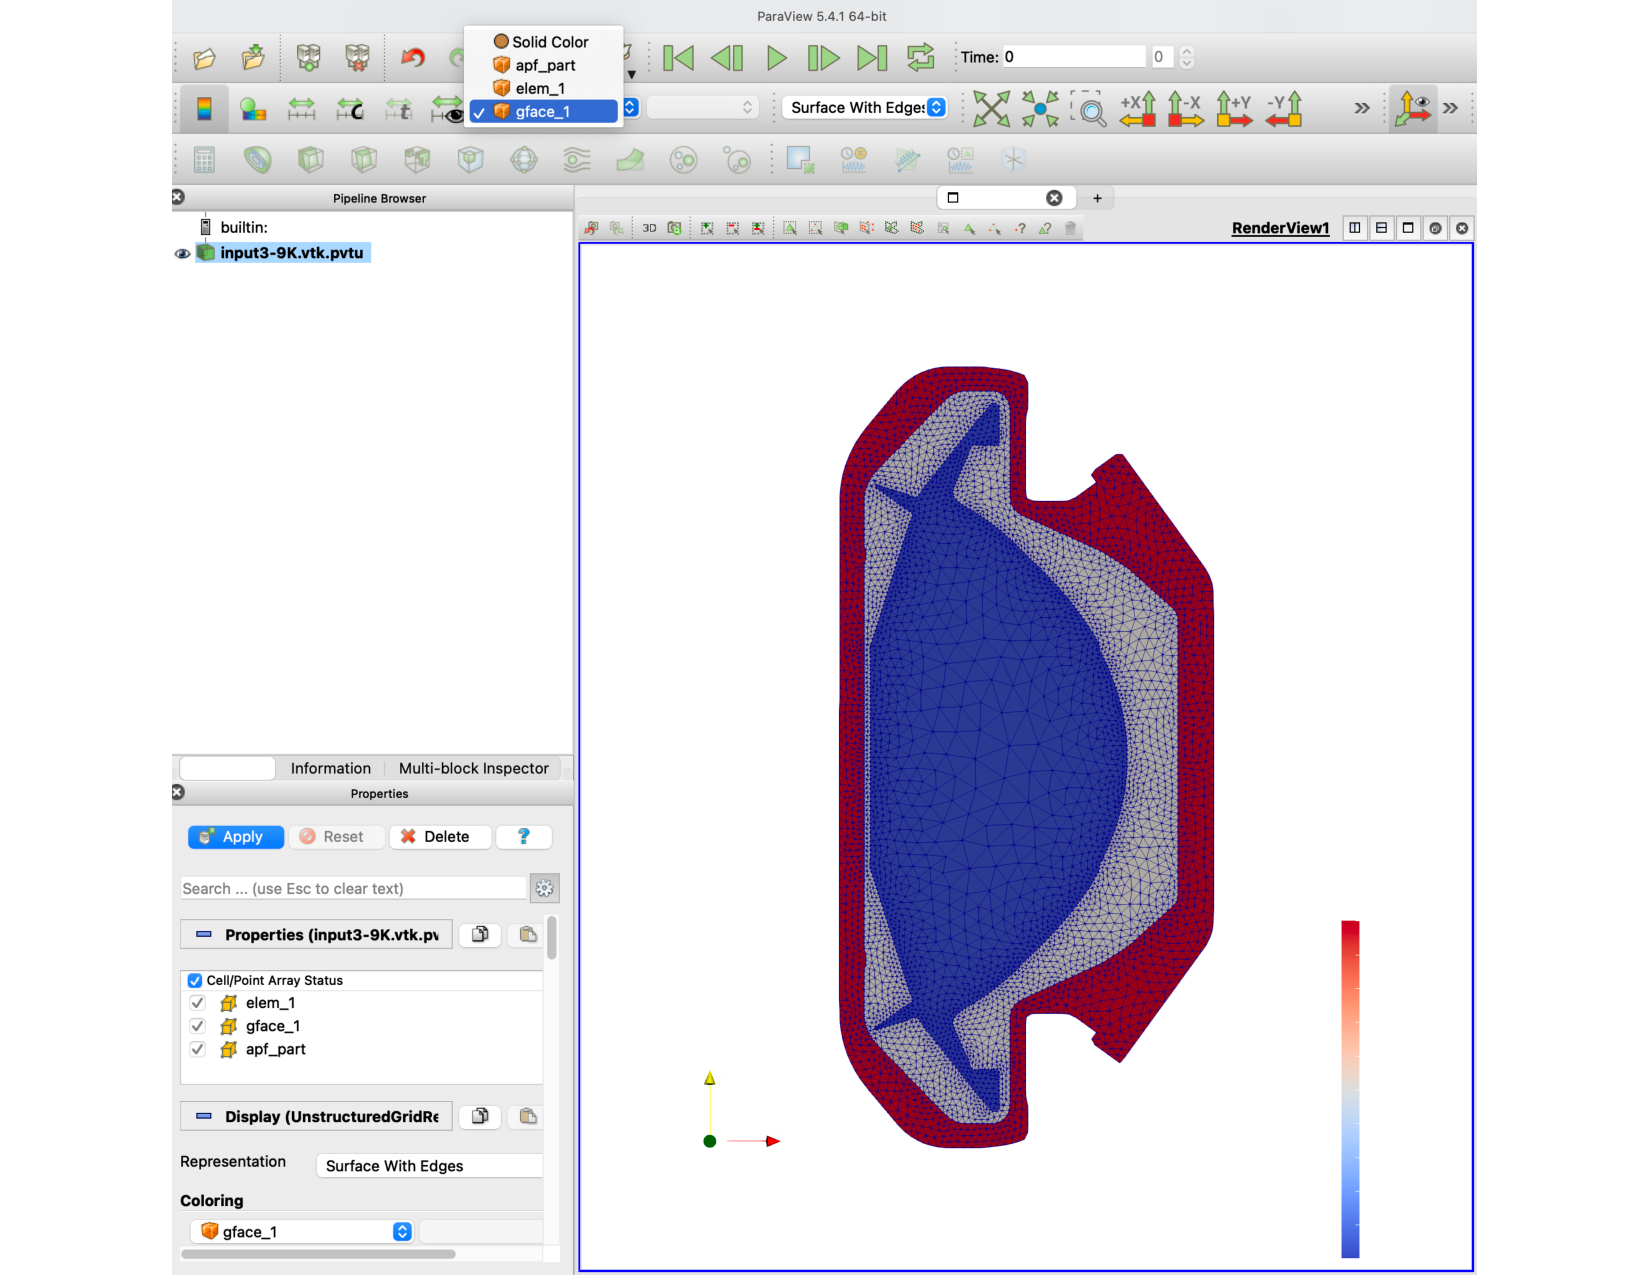
\includegraphics[width=4in]{./figures/paraview-fig5.pdf}
\caption{A mesh rendered with ``gface"}
\label{fig:paraview-5}
\end{figure}

Mesh generation program provides ``gface" alternative, which
allows users to see the geometric face of the mesh in color. 
Figure ~\ref{fig:paraview-5} depicts a Paraview window with a mesh rendered with ''gface".


\begin{figure}
\centering
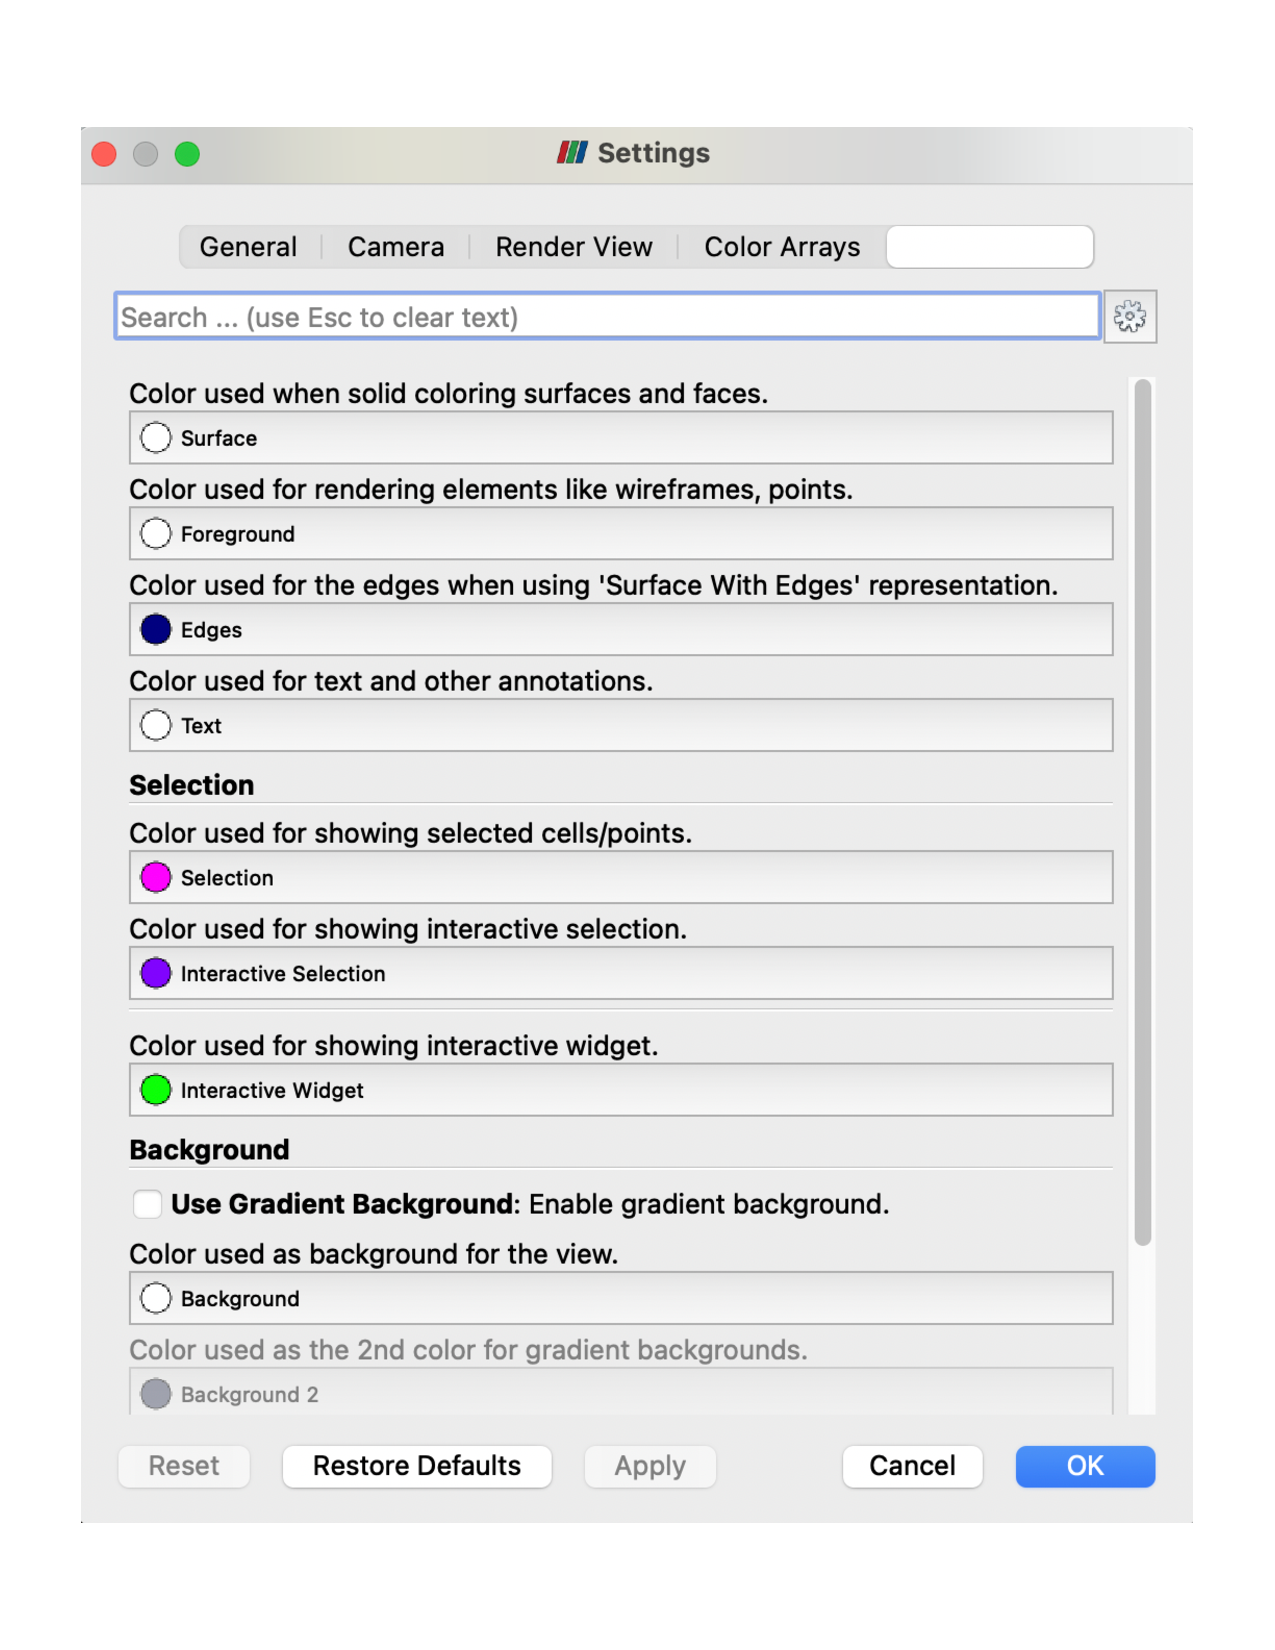
\includegraphics[width=3in]{./figures/paraview-fig6.pdf}
\caption{``Color Palette" tab of ``Settings" menu"}
\label{fig:paraview-6}
\end{figure}
Figure~\ref{fig:paraview-6} illustrates the ``Color Palette" tab of ``Settings" menu which allows the users to change the colors of ``Render View" such as edges, background, etc.. 
